% Options for packages loaded elsewhere
\PassOptionsToPackage{unicode}{hyperref}
\PassOptionsToPackage{hyphens}{url}
\PassOptionsToPackage{dvipsnames,svgnames,x11names}{xcolor}
%
\documentclass[
]{agujournal2019}

\usepackage{amsmath,amssymb}
\usepackage{iftex}
\ifPDFTeX
  \usepackage[T1]{fontenc}
  \usepackage[utf8]{inputenc}
  \usepackage{textcomp} % provide euro and other symbols
\else % if luatex or xetex
  \usepackage{unicode-math}
  \defaultfontfeatures{Scale=MatchLowercase}
  \defaultfontfeatures[\rmfamily]{Ligatures=TeX,Scale=1}
\fi
\usepackage{lmodern}
\ifPDFTeX\else  
    % xetex/luatex font selection
\fi
% Use upquote if available, for straight quotes in verbatim environments
\IfFileExists{upquote.sty}{\usepackage{upquote}}{}
\IfFileExists{microtype.sty}{% use microtype if available
  \usepackage[]{microtype}
  \UseMicrotypeSet[protrusion]{basicmath} % disable protrusion for tt fonts
}{}
\makeatletter
\@ifundefined{KOMAClassName}{% if non-KOMA class
  \IfFileExists{parskip.sty}{%
    \usepackage{parskip}
  }{% else
    \setlength{\parindent}{0pt}
    \setlength{\parskip}{6pt plus 2pt minus 1pt}}
}{% if KOMA class
  \KOMAoptions{parskip=half}}
\makeatother
\usepackage{xcolor}
\setlength{\emergencystretch}{3em} % prevent overfull lines
\setcounter{secnumdepth}{5}
% Make \paragraph and \subparagraph free-standing
\ifx\paragraph\undefined\else
  \let\oldparagraph\paragraph
  \renewcommand{\paragraph}[1]{\oldparagraph{#1}\mbox{}}
\fi
\ifx\subparagraph\undefined\else
  \let\oldsubparagraph\subparagraph
  \renewcommand{\subparagraph}[1]{\oldsubparagraph{#1}\mbox{}}
\fi

\usepackage{color}
\usepackage{fancyvrb}
\newcommand{\VerbBar}{|}
\newcommand{\VERB}{\Verb[commandchars=\\\{\}]}
\DefineVerbatimEnvironment{Highlighting}{Verbatim}{commandchars=\\\{\}}
% Add ',fontsize=\small' for more characters per line
\usepackage{framed}
\definecolor{shadecolor}{RGB}{241,243,245}
\newenvironment{Shaded}{\begin{snugshade}}{\end{snugshade}}
\newcommand{\AlertTok}[1]{\textcolor[rgb]{0.68,0.00,0.00}{#1}}
\newcommand{\AnnotationTok}[1]{\textcolor[rgb]{0.37,0.37,0.37}{#1}}
\newcommand{\AttributeTok}[1]{\textcolor[rgb]{0.40,0.45,0.13}{#1}}
\newcommand{\BaseNTok}[1]{\textcolor[rgb]{0.68,0.00,0.00}{#1}}
\newcommand{\BuiltInTok}[1]{\textcolor[rgb]{0.00,0.23,0.31}{#1}}
\newcommand{\CharTok}[1]{\textcolor[rgb]{0.13,0.47,0.30}{#1}}
\newcommand{\CommentTok}[1]{\textcolor[rgb]{0.37,0.37,0.37}{#1}}
\newcommand{\CommentVarTok}[1]{\textcolor[rgb]{0.37,0.37,0.37}{\textit{#1}}}
\newcommand{\ConstantTok}[1]{\textcolor[rgb]{0.56,0.35,0.01}{#1}}
\newcommand{\ControlFlowTok}[1]{\textcolor[rgb]{0.00,0.23,0.31}{#1}}
\newcommand{\DataTypeTok}[1]{\textcolor[rgb]{0.68,0.00,0.00}{#1}}
\newcommand{\DecValTok}[1]{\textcolor[rgb]{0.68,0.00,0.00}{#1}}
\newcommand{\DocumentationTok}[1]{\textcolor[rgb]{0.37,0.37,0.37}{\textit{#1}}}
\newcommand{\ErrorTok}[1]{\textcolor[rgb]{0.68,0.00,0.00}{#1}}
\newcommand{\ExtensionTok}[1]{\textcolor[rgb]{0.00,0.23,0.31}{#1}}
\newcommand{\FloatTok}[1]{\textcolor[rgb]{0.68,0.00,0.00}{#1}}
\newcommand{\FunctionTok}[1]{\textcolor[rgb]{0.28,0.35,0.67}{#1}}
\newcommand{\ImportTok}[1]{\textcolor[rgb]{0.00,0.46,0.62}{#1}}
\newcommand{\InformationTok}[1]{\textcolor[rgb]{0.37,0.37,0.37}{#1}}
\newcommand{\KeywordTok}[1]{\textcolor[rgb]{0.00,0.23,0.31}{#1}}
\newcommand{\NormalTok}[1]{\textcolor[rgb]{0.00,0.23,0.31}{#1}}
\newcommand{\OperatorTok}[1]{\textcolor[rgb]{0.37,0.37,0.37}{#1}}
\newcommand{\OtherTok}[1]{\textcolor[rgb]{0.00,0.23,0.31}{#1}}
\newcommand{\PreprocessorTok}[1]{\textcolor[rgb]{0.68,0.00,0.00}{#1}}
\newcommand{\RegionMarkerTok}[1]{\textcolor[rgb]{0.00,0.23,0.31}{#1}}
\newcommand{\SpecialCharTok}[1]{\textcolor[rgb]{0.37,0.37,0.37}{#1}}
\newcommand{\SpecialStringTok}[1]{\textcolor[rgb]{0.13,0.47,0.30}{#1}}
\newcommand{\StringTok}[1]{\textcolor[rgb]{0.13,0.47,0.30}{#1}}
\newcommand{\VariableTok}[1]{\textcolor[rgb]{0.07,0.07,0.07}{#1}}
\newcommand{\VerbatimStringTok}[1]{\textcolor[rgb]{0.13,0.47,0.30}{#1}}
\newcommand{\WarningTok}[1]{\textcolor[rgb]{0.37,0.37,0.37}{\textit{#1}}}

\providecommand{\tightlist}{%
  \setlength{\itemsep}{0pt}\setlength{\parskip}{0pt}}\usepackage{longtable,booktabs,array}
\usepackage{calc} % for calculating minipage widths
% Correct order of tables after \paragraph or \subparagraph
\usepackage{etoolbox}
\makeatletter
\patchcmd\longtable{\par}{\if@noskipsec\mbox{}\fi\par}{}{}
\makeatother
% Allow footnotes in longtable head/foot
\IfFileExists{footnotehyper.sty}{\usepackage{footnotehyper}}{\usepackage{footnote}}
\makesavenoteenv{longtable}
\usepackage{graphicx}
\makeatletter
\def\maxwidth{\ifdim\Gin@nat@width>\linewidth\linewidth\else\Gin@nat@width\fi}
\def\maxheight{\ifdim\Gin@nat@height>\textheight\textheight\else\Gin@nat@height\fi}
\makeatother
% Scale images if necessary, so that they will not overflow the page
% margins by default, and it is still possible to overwrite the defaults
% using explicit options in \includegraphics[width, height, ...]{}
\setkeys{Gin}{width=\maxwidth,height=\maxheight,keepaspectratio}
% Set default figure placement to htbp
\makeatletter
\def\fps@figure{htbp}
\makeatother
% definitions for citeproc citations
\NewDocumentCommand\citeproctext{}{}
\NewDocumentCommand\citeproc{mm}{%
  \begingroup\def\citeproctext{#2}\cite{#1}\endgroup}
\makeatletter
 % allow citations to break across lines
 \let\@cite@ofmt\@firstofone
 % avoid brackets around text for \cite:
 \def\@biblabel#1{}
 \def\@cite#1#2{{#1\if@tempswa , #2\fi}}
\makeatother
\newlength{\cslhangindent}
\setlength{\cslhangindent}{1.5em}
\newlength{\csllabelwidth}
\setlength{\csllabelwidth}{3em}
\newenvironment{CSLReferences}[2] % #1 hanging-indent, #2 entry-spacing
 {\begin{list}{}{%
  \setlength{\itemindent}{0pt}
  \setlength{\leftmargin}{0pt}
  \setlength{\parsep}{0pt}
  % turn on hanging indent if param 1 is 1
  \ifodd #1
   \setlength{\leftmargin}{\cslhangindent}
   \setlength{\itemindent}{-1\cslhangindent}
  \fi
  % set entry spacing
  \setlength{\itemsep}{#2\baselineskip}}}
 {\end{list}}
\usepackage{calc}
\newcommand{\CSLBlock}[1]{\hfill\break\parbox[t]{\linewidth}{\strut\ignorespaces#1\strut}}
\newcommand{\CSLLeftMargin}[1]{\parbox[t]{\csllabelwidth}{\strut#1\strut}}
\newcommand{\CSLRightInline}[1]{\parbox[t]{\linewidth - \csllabelwidth}{\strut#1\strut}}
\newcommand{\CSLIndent}[1]{\hspace{\cslhangindent}#1}

\usepackage{url} %this package should fix any errors with URLs in refs.
\usepackage{lineno}
\usepackage[inline]{trackchanges} %for better track changes. finalnew option will compile document with changes incorporated.
\usepackage{soul}
\linenumbers
\makeatletter
\@ifpackageloaded{caption}{}{\usepackage{caption}}
\AtBeginDocument{%
\ifdefined\contentsname
  \renewcommand*\contentsname{Table of contents}
\else
  \newcommand\contentsname{Table of contents}
\fi
\ifdefined\listfigurename
  \renewcommand*\listfigurename{List of Figures}
\else
  \newcommand\listfigurename{List of Figures}
\fi
\ifdefined\listtablename
  \renewcommand*\listtablename{List of Tables}
\else
  \newcommand\listtablename{List of Tables}
\fi
\ifdefined\figurename
  \renewcommand*\figurename{Figure}
\else
  \newcommand\figurename{Figure}
\fi
\ifdefined\tablename
  \renewcommand*\tablename{Table}
\else
  \newcommand\tablename{Table}
\fi
}
\@ifpackageloaded{float}{}{\usepackage{float}}
\floatstyle{ruled}
\@ifundefined{c@chapter}{\newfloat{codelisting}{h}{lop}}{\newfloat{codelisting}{h}{lop}[chapter]}
\floatname{codelisting}{Listing}
\newcommand*\listoflistings{\listof{codelisting}{List of Listings}}
\makeatother
\makeatletter
\makeatother
\makeatletter
\@ifpackageloaded{caption}{}{\usepackage{caption}}
\@ifpackageloaded{subcaption}{}{\usepackage{subcaption}}
\makeatother
\ifLuaTeX
  \usepackage{selnolig}  % disable illegal ligatures
\fi
\usepackage{bookmark}

\IfFileExists{xurl.sty}{\usepackage{xurl}}{} % add URL line breaks if available
\urlstyle{same} % disable monospaced font for URLs
\hypersetup{
  pdftitle={Analysis of Methylated DNA},
  pdfauthor={Piero Palacios Bernuy},
  pdfkeywords={450k array, methylation, CpG, CpGs islands},
  colorlinks=true,
  linkcolor={blue},
  filecolor={Maroon},
  citecolor={Blue},
  urlcolor={Blue},
  pdfcreator={LaTeX via pandoc}}

\journalname{An open source portfolio}

\draftfalse

\begin{document}
\title{Analysis of Methylated DNA}

\authors{Piero Palacios Bernuy\affil{}}

\correspondingauthor{Piero Palacios Bernuy}{p.palacios.bernuy@gmail.com}


\begin{abstract}
This document is part of a series of the analysis of Omics data.
Especifycally, here is showed how to analyze Illumina 450k array and
Methyl-Seq data with Bioconductor packages. Also, it's showcased how to
make plots of the methylation data in the context of genomic positions
and genes strutctures.
\end{abstract}

\section*{Plain Language Summary}
This document have examples of the analysis of Illumina 450k array and
Methyl-Seq data.



\section{Methylation analysis}\label{methylation-analysis}

\subsection{Methylation}\label{methylation}

Epigenetics is the study of how your behaviors and environment can cause
changes that affect the way your genes work. Unlike genetic changes,
epigenetic changes are reversible and do not change your DNA sequence,
but they can change how your body reads a DNA sequence (CDC,2024).

Talking about the genes, these can only be expressed when the chromatin
is in it's relaxed form (euchromatin) and reversely, these cannot be
expressed in it's compacted form (hetero-chromatin). Methylation of
cytosine's control part of this process of the chromatin and it's really
important to understand is a gene (or the surroundings) is methylated.

\begin{figure}[H]

{\centering \includegraphics[width=4.65625in,height=\textheight]{index_files/mediabag/urn-cambridge.org-id.png}

}

\caption{DNA Methylation}

\end{figure}%

\subsection{CpG's}\label{cpgs}

The cytosine's (C) that are methylated are followed by a guanine (G).
This pattern is called CpG in the context of epigenetics. These CpG's
tend to cluster into groups (CpG islands) and, these Cpg islands tend to
be close to the promoter region of the genes.

\subsection{Bisulfite treatment}\label{bisulfite-treatment}

\begin{figure}[H]

{\centering \includegraphics{index_files/mediabag/bisulfite.png}

}

\caption{Bisulfite Treatment}

\end{figure}%

If a C is methylated the bisulfite treatment won´t change the cytosine
but, if the C is not methylated, the C will suffer a transition to a T.

\subsection{Methylation 450k array}\label{methylation-450k-array}

To see how to analyze from a Illumina 450k array with the (Fortin et
al., 2016) package, click to the script below the image.

\begin{figure}[H]

\centering{

\captionsetup{labelsep=none}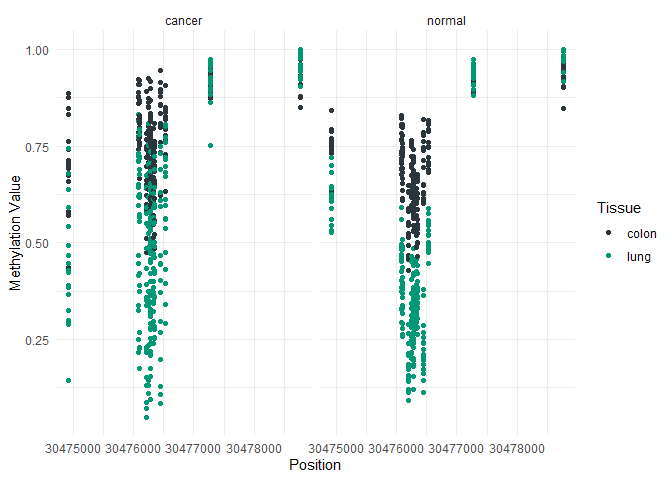
\includegraphics{index_files/figure-latex/notebooks-Methylation_analysis-fig-meth-output-1.png}

}

\caption{\label{fig-meth}}

\end{figure}%

\textsubscript{Source:
\href{https://pipaber.github.io/Epigenomics/notebooks/Methylation_analysis-preview.html\#cell-fig-meth}{DNA
methylation measurement}}

\subsection{Methylation 450k array - Multi-resolution
Analysis}\label{methylation-450k-array---multi-resolution-analysis}

To see how to analyze at a multi-resolution level from a Illumina 450k
array with the (Fortin et al., 2016) package, click to the script below
the table.

\begin{figure}[H]

{\centering 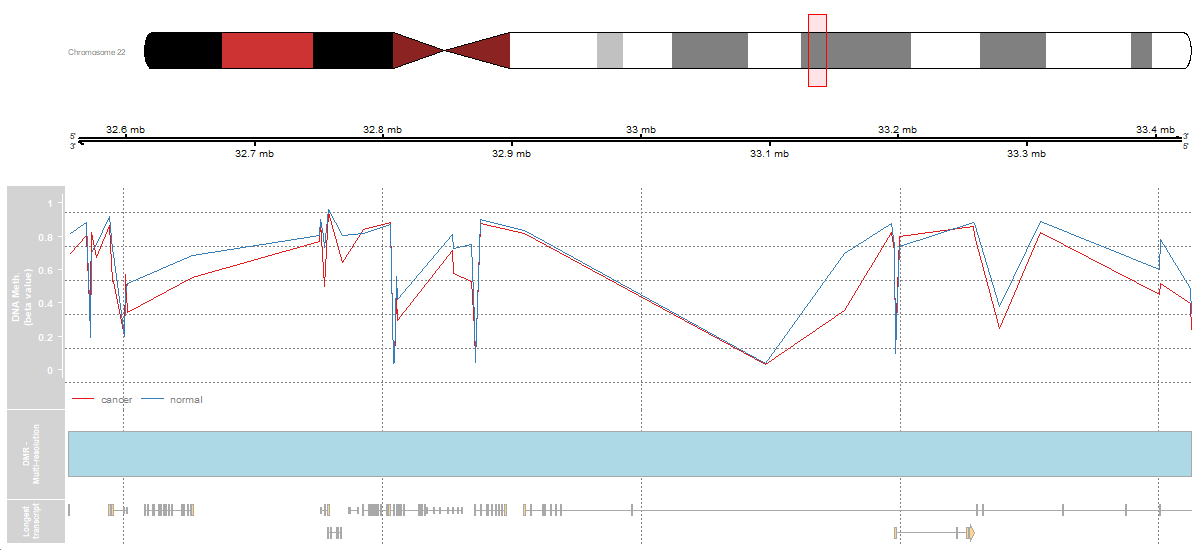
\includegraphics{notebooks/track_plot.png}

}

\caption{Methylation DMR}

\end{figure}%

\begin{Shaded}
\begin{Highlighting}[]
\NormalTok{mcols(granges(dat$object))$type }\OperatorTok{|\textgreater{}} 
\NormalTok{    table() }\OperatorTok{|\textgreater{}} 
\NormalTok{    prop.table() }\OperatorTok{|\textgreater{}} 
    \ImportTok{as}\NormalTok{.data.frame() }\OperatorTok{|\textgreater{}} 
\NormalTok{    dplyr::rename(}\StringTok{"Island Status"} \OperatorTok{=}\NormalTok{ Var1) }\OperatorTok{|\textgreater{}} 
\NormalTok{    gt::gt()}
\end{Highlighting}
\end{Shaded}

\phantomsection\label{island-status}
\begin{longtable}[]{@{}ll@{}}
\toprule\noalign{}
Island Status & Freq \\
\midrule\noalign{}
\endhead
\bottomrule\noalign{}
\endlastfoot
Island & 0.1811251 \\
OpenSea & 0.2134595 \\
Shelf & 0.2705047 \\
Shore & 0.3349106 \\
\end{longtable}

\textsubscript{Source:
\href{https://pipaber.github.io/Epigenomics/notebooks/Methylation_multiresolution_analysis-preview.html\#cell-Island-status}{DNA
methylation measurement}}

\section{Methyl-Seq}\label{methyl-seq}

Analyzing bisulfite sequencing data requires a server or an HPC. U can
use the \emph{methylseq} pipeline from
\href{https://nf-co.re/methylseq/2.6.0}{nfcore} to get the .cov files to
proced with the downstream analysis on R.

To see how to analyze Whole-genome bisulfite sequencing (WGBS) with the
(Hansen et al., 2012), click on the script below the image.

\subsection{WGBS}\label{wgbs}

\begin{figure}[H]

{\centering 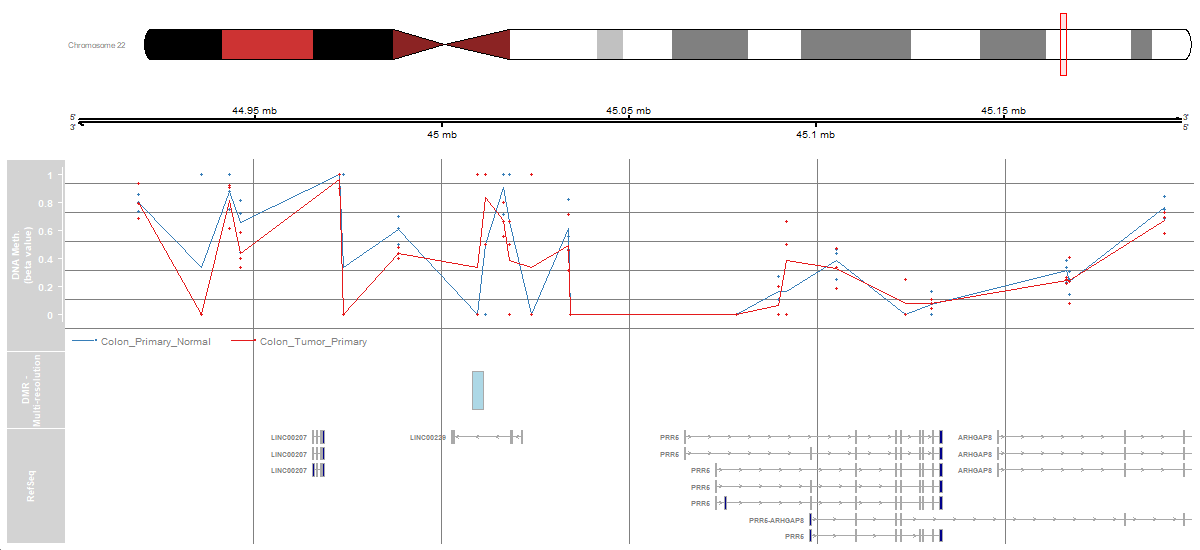
\includegraphics{notebooks/track_methyl_seq_plot.png}

}

\caption{Methylation DMR}

\end{figure}%

\begin{figure}[H]

\centering{

\captionsetup{labelsep=none}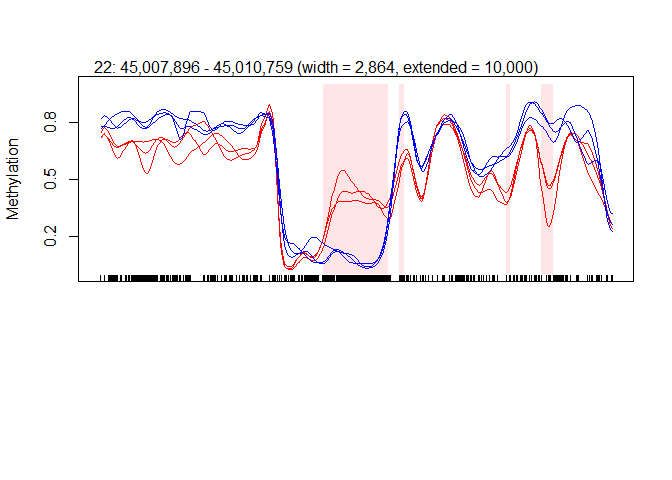
\includegraphics{index_files/figure-latex/notebooks-Methyl_Seq-fig-dmr-output-1.png}

}

\caption{\label{fig-dmr}}

\end{figure}%

\textsubscript{Source:
\href{https://pipaber.github.io/Epigenomics/notebooks/Methyl_Seq-preview.html\#cell-fig-dmr}{DNA
methylation measurement by sequencing}}

\section*{References}\label{references}
\addcontentsline{toc}{section}{References}

\phantomsection\label{refs}
\begin{CSLReferences}{1}{0}
\vspace{1em}

\bibitem[\citeproctext]{ref-minfi}
Fortin, J.-P., Triche, J., Timothy J., \& Hansen, K. D. (2016).
{Preprocessing, normalization and integration of the Illumina
HumanMethylationEPIC array with minfi}. \emph{Bioinformatics},
\emph{33}(4), 558--560.
\url{https://doi.org/10.1093/bioinformatics/btw691}

\bibitem[\citeproctext]{ref-bsseq}
Hansen, K. D., Langmead, B., \& Irizarry, R. A. (2012).
{\textbraceleft}BSmooth: From whole genome bisulfite sequencing reads to
differentially methylated regions{\textbraceright}, \emph{13}, R83.
\url{https://doi.org/10.1186/gb-2012-13-10-r83}

\end{CSLReferences}



\end{document}
